\documentclass{article}

\usepackage{
    amsmath
,   physics
,   microtype
,   graphicx
,   enumitem
,   gensymb
,   tikz
,   color
,   etoolbox
,   fancyhdr
}
\usepackage[letterpaper, top=1in, bottom=1in, left=1in, right=1in]{geometry}

\pagestyle{fancy}

\patchcmd\subequations{\alph}{\Alph}{}{}{}
\usepackage{hyperref}

\title{Kinematic Practice Problems}
\author{Laith Toom}
\date{24/2/2023}

\begin{document}
\maketitle
\newpage
\tableofcontents
\newpage

\section{Chapter 2: 1D Motion}

    \subsection{Problem 34: Page 34}
    A red car and a green car, identical except for the 
    color, move toward each other in adjacent lanes and 
    parallel to an $x$ acis. At time $t=0$, the red car 
    is at $x_r=0$ and the green car is at $x_g=220\,\mathrm{m}$.
    If the red car has a constant velocity of $20\,\mathrm{km/h}$,
    the cars pass each other at $x=44.5\,\mathrm{m}$, and if it has 
    a constant velocity of $40\,\mathrm{km/h}$, they pass each other at
    $x=76.6\,\mathrm{m}$. What are:
    \begin{enumerate}[label=(\alph*)]
        \item the initial velocity 
        \item the constant acceleration
    \end{enumerate}
    of the green car?
    \begin{figure}[h!]
        \centering 
        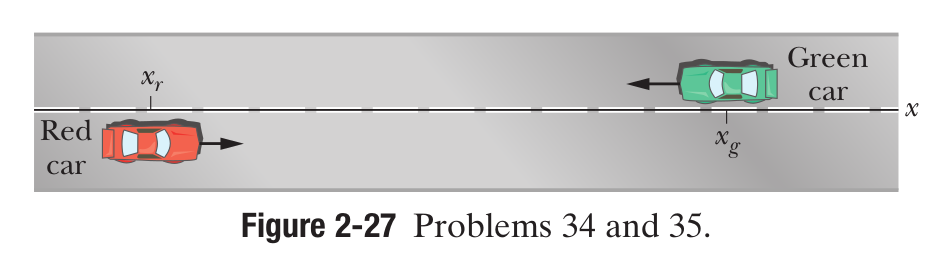
\includegraphics[width=10cm]{Exam1Practice_Figures/fig34_34.png}
    \end{figure}
    \begin{subequations}

    \subsubsection{Solution}
    We can define the positions of the red car and green car as 
    functions of time:
    \begin{gather*}
        x_r(t) - x_r = v_rt \tag{R}\\ 
        \intertext{The acceleration of the red car is 0 because its velocity is constant.}
        x_g(t) - x_g = v_0t + \frac{1}{2}at^2 \tag{G}
    \end{gather*}

    We know that the initial position of the red car, $x_r$, is 0 m and the initial 
    position of the green car, $x_g$, is 220 m, thus:
    \begin{gather*}
        x_r(t) = v_rt \\
        x_g(t) - 220 = v_0t + \frac{1}{2}at^2
    \end{gather*}

    Since we are given two scenarios, in which the velocity of the red car and the 
    position at which the two cars meet change, but the initial velocity and acceleration 
    of the green car remain the same, we can set up a system of equations to solve for 
    $v_0$ and subsequently $a$ of the green car:
    \begin{gather}
        \intertext{If the velocity of the red car is $\frac{50}{9}$ m/s, then both cars 
        meet at 44.5 m. We can solve for time $t_1$:}
        x_r(t_1) = 44.5 \implies 44.5 = \frac{50}{9}t_1 \\
        \Rightarrow t_1 = 8.01    
        \intertext{We can do the same if $v_r = \frac{100}{9}$, in which the position 
        is now 76.6 m. We can solve for time $t_1$:}
        x_r(t_2) = 76.6 \implies 76.6 = \frac{100}{9}t_2 \\
        \Rightarrow t_2 = 6.89
        \intertext{We can plug both times into our function $x_g(t)$ to get 
        a system of two equations:}
        x_g(t_1) - 220 = 44.5 - 220 = -175.5 \implies -175.5 = v_0t_1 + \frac{1}{2}at_1^2 \\
        x_g(t_2) - 220 = 76.6.5 - 220 = -143.4 \implies -143.4 = v_0t_2 + \frac{1}{2}at_2^2
        \intertext{We can solve for $a$ in equation 1E and plug that value into equation 
        $1F$ to solve for $v_0$:}
        a = \frac{2}{t_1^2}\left( -175.5-v_0t_1 \right) \\
        \implies -143.4 = v_0t_2 + \frac{1}{2}\left( \frac{2}{t_1^2}\left( -175.5-v_0t_1 \right)  \right)t_2^2 \\
        \Rightarrow -143.4 = v_0t_2 + \frac{t_2^2}{t_1^2}\left( -175.5 - v_0t_1 \right) \nonumber \\
        \Rightarrow -143.4 = t_2\left(v_0 + \frac{t_2}{t_1^2}\left( -175.5 - v_0t_1 \right)\right) \nonumber \\
        \Rightarrow -143.4 = t_2\left(v_0 + \frac{t_2}{t_1^2}(-175.5) - v_0\frac{t_2}{t_1} \right) \nonumber \\
        \Rightarrow -143.4 = t_2\left( \left( 1-\frac{t_2}{t_1} \right)v_0 + \frac{t_2}{t_1^2}(-175.5) \right) \nonumber \\
        \Rightarrow \frac{-143.4}{t_2} = \left( 1-\frac{t_2}{t_1} \right)v_0 + \frac{t_2}{t_1^2}(-175.5) \nonumber \\
        \Rightarrow \frac{-143.4}{t_2} - \frac{t_2}{t_1^2}(-175.5) = \left( 1-\frac{t_2}{t_1} \right)v_0  \nonumber \\
        \Rightarrow v_0 = \dfrac{\dfrac{-143.4}{t_2} - \dfrac{t_2}{t_1^2}(-175.5)}{1-\dfrac{t_2}{t_1}} \nonumber
        \intertext{Substituting in our parameters, we get:}
        v_0 = \dfrac{\dfrac{-143.4}{6.89} - \dfrac{6.89}{8.01^2}(-175.5)}{1-\dfrac{6.89}{8.01}} \\
        \boxed{ v_0 \approx -14.06 \,\mathrm{m/s} } \tag{a}
        \intertext{Now we can substitute this value into equation 1G to solve for $a$:}
        a = \frac{2}{8.01^2}[-175.5+14.06(8.01)] \approx -1.92 \,\mathrm{m/s}^2 \\
        \boxed { a \approx -1.92 \,\mathrm{m/s}^2 }
    \end{gather}

    \end{subequations}

\newpage

\section{Chapter 3: Vectors}

    % \subsection{Problem 29: Page 58}
    % Typical backyard ants often create a network of chemical 
    % trails for guidance. Extending outward from the nest, a trail
    % branches (\textit{bifurcates}) repeatedly, with $60\degree$
    % between the branches. If a roaming ant chances upon a trail, it 
    % can tell the way to the nest at any branch point: If it is moving 
    % awat from the nest, it has two choices of path requiring a small turn 
    % in its travel direction, either $30\degree$ leftward or $30\degree$
    % rightward. If it is moving toward the nest, it has only one such choice. 
    % Figure 3-29 shows a typical ant trail, with lettered straight sections
    % of $2.0\,\mathrm{cm}$ length and symmetric bifurcation of $60\degree$.
    % Path $v$ is parallel to the $y$ axis. What are the:
    % \begin{enumerate}[label=(\alph*)]
    %     \item magnitude
    %     \item angle
    % \end{enumerate}
    % (relative to the positive direction of the superimposed $x$ axis) of 
    % an ant's displacement from the nest (find it in the figure) if the ant 
    % enters the trail at point $A$? What are the:
    % \begin{enumerate}[label=(\alph*), start=3]
    %     \item magnitude
    %     \item angle
    % \end{enumerate}
    % if it enters at point $B$?
    % \begin{figure}[h!]
    %    \centering 
    %    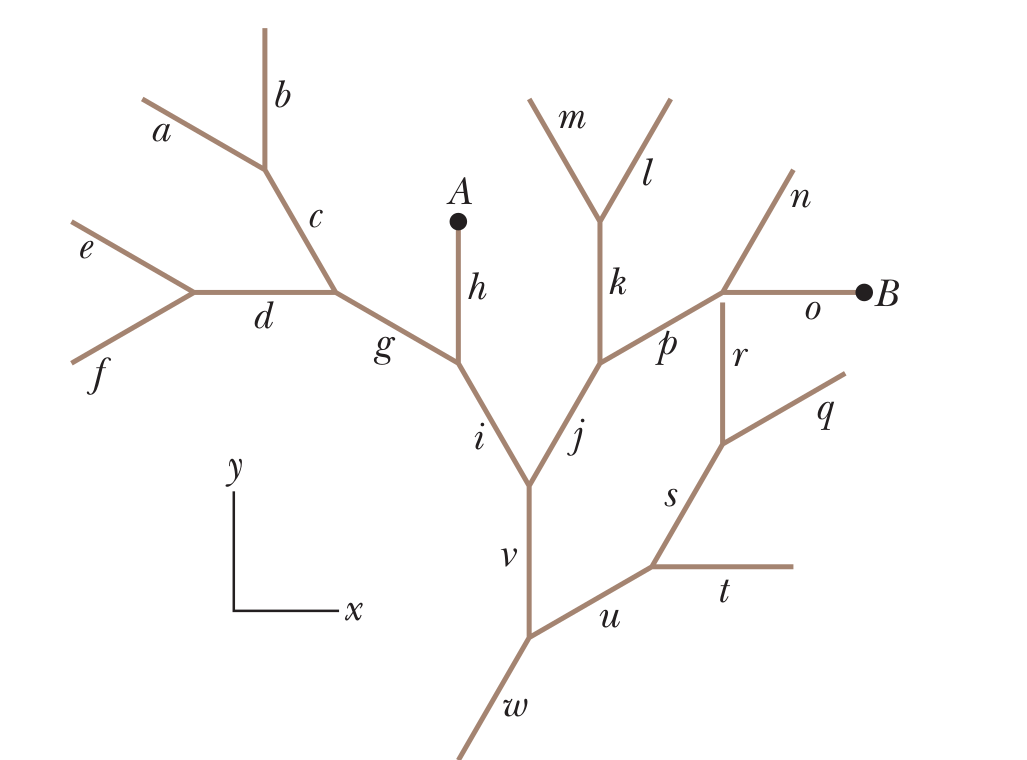
\includegraphics[width=10cm]{Exam1Practice_Figures/vector.png}
    %    \caption{3-29}
    % \end{figure}
    % \begin{subequations}
    
    % \subsubsection{Solution}

    % \end{subequations}

    \newpage

    \subsection{Problem 31: Page 58}
    In Fig. 3-30, a vector $\va{a}$ with a magnitude 
    of $17.0\,\mathrm{m}$ is directed at angle $\theta=56.0\degree$
    counterclockwise from the $+x$ axis. What are the 
    components (a) $a_x$ and (b) $a_y$ of the vector? A 
    second coordinate system is inclined by angle $\theta'=18.0\degree$
    with respect to the first. What are the components (c) $a'_x$ 
    and (d) $a'_y$ in this primed coordinate system?
    \begin{figure}[h!]
        \centering
        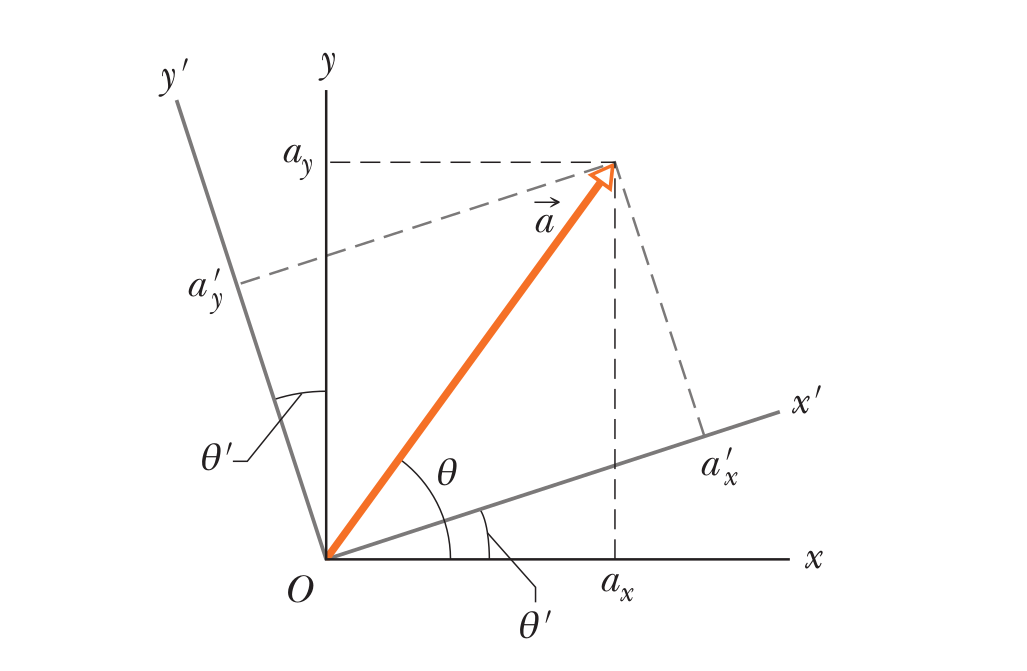
\includegraphics[width=10cm]{Exam1Practice_Figures/vector2.png}
        \caption{3-30}
    \end{figure}
    \begin{subequations}
    
    \subsubsection{Solution}
    We can draw a triangle using $\theta$ to solve for the components using 
    trig functions:
    \begin{gather}
        \cos(\theta) = \frac{a_x}{\va{a}} \implies \boxed{ a_x =  \va{a}\cos(\theta) } \tag{a} \\
        \sin(\theta) = \frac{a_y}{\va{a}} \implies \boxed{ a_y = \va{a}\sin(\theta) } \tag{b}
    \end{gather}
    We can draw another triangle using $\theta'$ to solve for the other components:
    \begin{gather}
        \cos(\theta') = \frac{a_x'}{\va{a}} \implies \boxed{ a_x' = \va{a}\cos(\theta') } \tag{c} \\
        \sin(\theta') = \frac{a_y'}{\va{a}} \implies \boxed{ a_y' = \va{a}\sin(\theta') } \tag{d}
    \end{gather}
    \end{subequations}

\newpage

\section{Chapter 4: 2D and 3D Motion}

    \subsection{Problem 38: Page 86}
    A golf ball is struck at ground level. The speed of the golf 
    ball is a function of the time is shown in Fig. 4-36, where 
    $t=0$ at the instant the ball is struck. The scaling on the vertical 
    axis is set by $v_a=19\,\mathrm{m/s}$ and $v_b=31\,\mathrm{m/s}$.
    \begin{enumerate}[label=(\alph*)]
        \item How far does the golf ball travel 
        horizontally before returning to ground level?
        \item What is the maximum height above the ground 
        level attained by the ball?
    \end{enumerate}
    \begin{figure}[h!]
        \centering    
        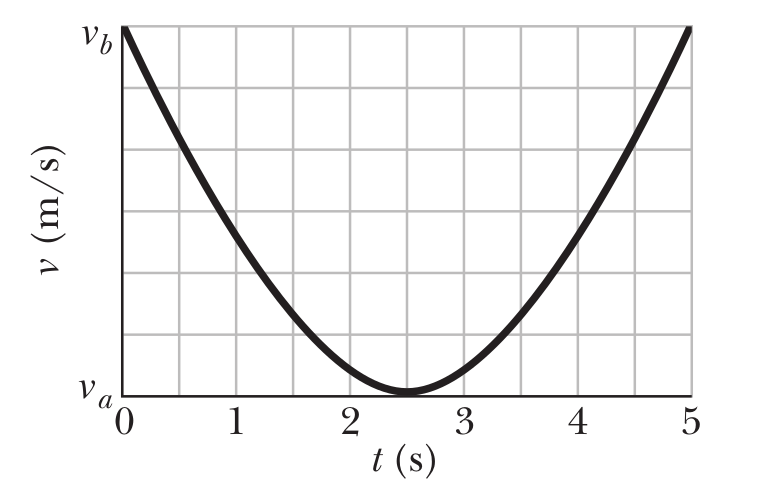
\includegraphics[width=10cm]{Exam1Practice_Figures/motion.png}
    \end{figure}
    \begin{subequations}
    
    \subsubsection{Solution}
    Looking at the graph, we can tell that the ball returns to the ground at $t=5$ 
    since it will travel with the same speed (magnitude of velocity) from 0 to 2.5 s 
    as it does from 2.5 to 5 s, only this time, the ball is traveling downwards instead
    of upwards. There is vertical acceleration due to gravity, so we need to use the 
    following equation:
    \[ \Delta{r} = vt-\frac{1}{2}at^2 \]
    there will be two different displacements, horizontal and vertical, thus we will have 
    2 different equations:
    \begin{gather}
        \Delta{r_y} = v_yt-\frac{1}{2}gt^2 \tag{vertical} \\
        \Delta{r_x} = v_xt \tag{horizontal}
    \end{gather}
    we can assume that horizontal acceleration is 0.
    
    \bigskip 

    Since the ball reaches its maximum height at $t=2.5$, the vertical velocity 
    at this moment is 0, thus:
    \begin{gather}
        \Delta{r_y} = (0)(2.5)-\frac{1}{2}g(2.5)^2 = \boxed{ 30.625 \,\mathrm{m} }
    \end{gather}
    Since there is no horizontal acceleration, the horizontal velocity is constant, 
    and we can solve for this component of velocity by taking the magnitude of 
    velocity when $v_y=0$, which as we established, occurs when the ball reaches 
    its maximum height at $t=2.5$:
    \begin{gather}
        \va{v}(2.5) = \sqrt{v_y(2.5)^2+v_x^2} \\
        \Rightarrow 19 = \sqrt{0+v_x^2} \implies v_x = 19 \\
        \Delta{r_x} = (19)(5) = \boxed{ 95 \,\mathrm{m} }
    \end{gather}
    \end{subequations}

    \newpage

    \subsection{Problem 71: Page 88}
    A suspicious-looking man runs as fast as he can along a moving 
    sidewalk from one end to the other, taking $2.50\,\mathrm{s}$. Then 
    security agents appear, and the man runs as fast as he can back 
    along the sidewalk to his starting point, taking $10.0\,\mathrm{s}$.
    What is the ratio of the man's running speed to the sidewalk's speed?
    \begin{subequations}
    
    \subsubsection{Solution}
    \end{subequations}

\newpage

\section{Chapter 5: Force and Motion}
    \subsection{Problem 34: Page 119}
    In Fig. 5-40, a crate of mass $m=100\,\mathrm{kg}$ is 
    pushed at constant speed up a frictionless ramp ($\theta=30.0\degree$)
    by a horizontal force $\va{F}$. What are the magnitudes of:
    \begin{enumerate}[label=(\alph*)]
        \item $\va{F}$
        \item the force on the crate from the ramp?
    \end{enumerate}
    \begin{figure}[h!]
        \centering 
        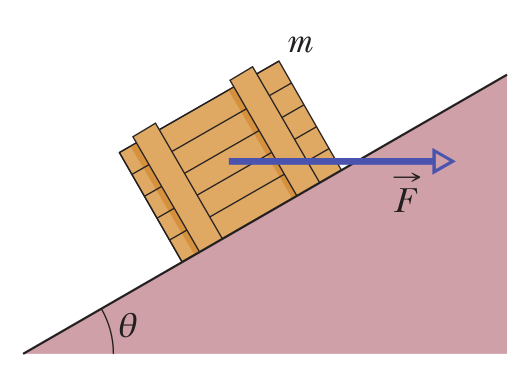
\includegraphics[width=10cm]{Exam1Practice_Figures/force.png}
    \end{figure}
    \begin{subequations}
    
    \subsubsection{Solution}
    We can draw a freebody diagram, with the center of the box being our 
    origin.
    \begin{figure}[h!]
        \centering 
        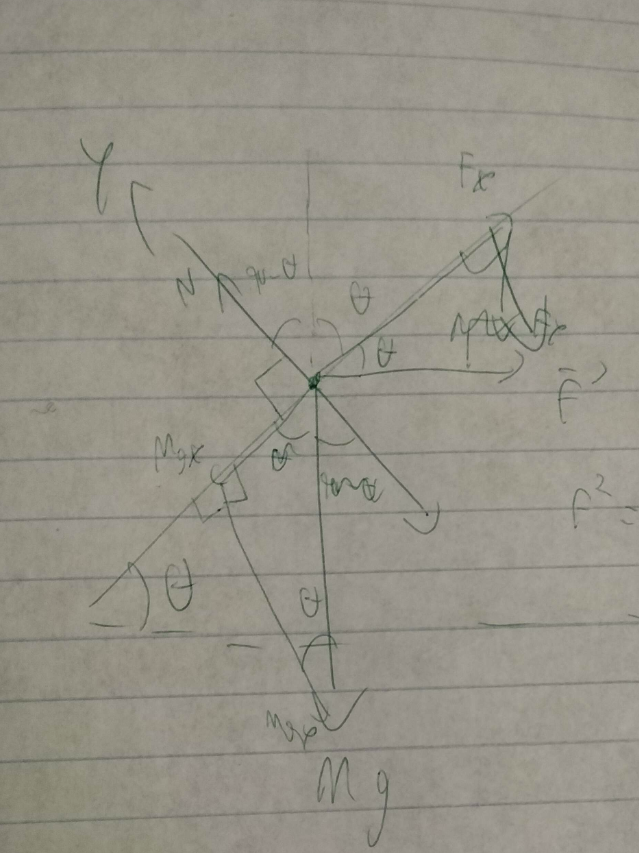
\includegraphics[width=5cm]{Exam1Practice_Figures/freebody.png}
    \end{figure}

    We can use $\theta$ to find the components of $\va{F}$ and $mg$ along the 
    $x$-axis since the components will form right triangles. You will see this 
    when you draw the diagram.

    Since we have no way of determing the normal force, we should solve for $\va{F}$ 
    by determing the net force along the $x$-axis:
    \begin{gather}
        \sin(\theta) = \frac{mg_x}{mg} \implies mg_x = mg\sin(\theta) \\
        \cos(\theta) = \frac{F_x}{\va{F}} \implies F_x = \va{F}\cos(\theta) \\
        x:\ \va{F}\cos(\theta) - mg\sin(\theta)
        \intertext{Since $F=ma$ and the box is moving with constant speed, we can 
        say that acceleration is 0, thus the net force is equal to $m(0)=0$:}
        \va{F}\cos(\theta) - mg\sin(\theta) = 0 \implies \boxed{\va{F} = mg\tan(\theta)}
    \end{gather}
    Now that we have $\va{F}$, we can calculate normal force $\va{N}$ by determing all of 
    components of force along the $y$-axis. Since the box is not moving along the $y$-axis, 
    we know the sum of forces along the $y$-axis will be 0:
    \begin{gather}
        \cos(\theta) = \frac{mg_y}{mg} \implies mg_y = mg\cos(\theta) \\
        \sin(\theta) = \frac{F_y}{\va{F}} \implies F_y = \va{F}\sin(\theta) \\
        y:\ \va{N} - mg\tan(\theta)\sin(\theta) - mg\cos(\theta) = 0 \\
        \implies \boxed{\va{N} = mg\tan(\theta)\sin(\theta) + mg\cos(\theta)}
    \end{gather}
    \end{subequations}

    \newpage

    \subsection{Problem 39: Page 119}
    A sphere of mass $3.0\times10^{-4}\,\mathrm{kg}$ is suspended 
    from a cord. A steady horizontal breeze pushes the sphere so that 
    the cord makes a constant angle of $37\degree$ with the vertical. Find:
    \begin{enumerate}[label=(\alph*)]
        \item the push magnitude
        \item the tension in the cord
    \end{enumerate} 
    \begin{subequations}
    
    \subsubsection{Solution}
    \end{subequations}

    \newpage

    \subsection{Problem 40: Page 119}
    A dated box of dates, of mass $5.00\,\mathrm{kg}$, is sent 
    sliding up a frictionless ramp at an angle of $\theta$ to 
    the horizontal. Figure 5-41 gives,
    \begin{figure}[h!]
        \centering 
        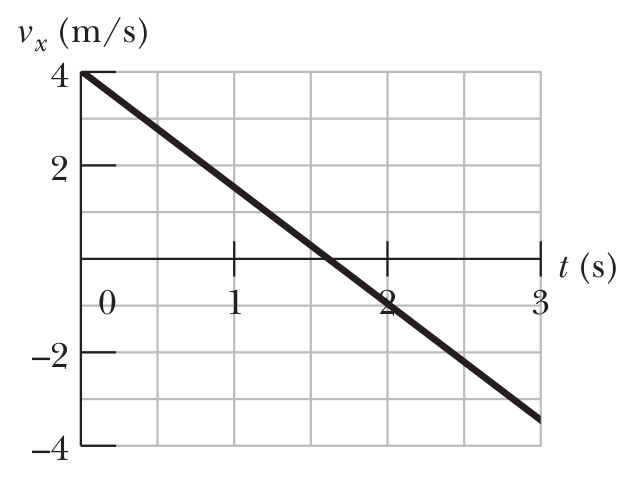
\includegraphics[width=10cm]{Exam1Practice_Figures/force2.png}
        \caption{5-41}
    \end{figure}
    as a function of time $t$, the component $v_x$ of the box's velocity 
    along an $x$ axis that extends directly up the ramp. What is the magnitude 
    of the normal force on the box from the ramp?
    \begin{subequations}
    
    \subsubsection{Solution}
    \end{subequations}

\end{document}